
\subsection{Principe de modélisation autonome}

\begin{figure}
  \centering
  \subfloat[Construction suivant une démarche linéaire]{
    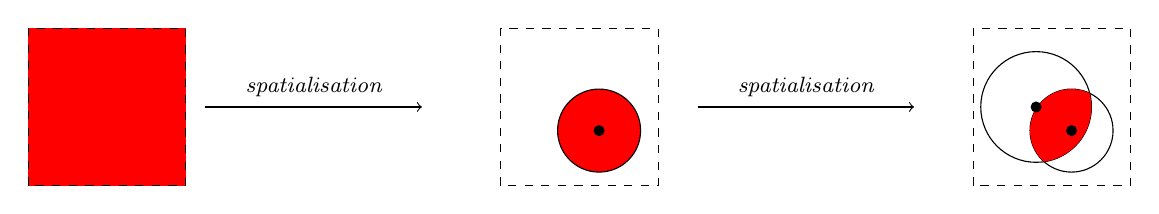
\begin{tikzpicture}

  \begin{scope}
    \path[fill=red] (0,0) rectangle (2,2);
	\path[draw, dashed] (0,0) rectangle (2,2);
  \end{scope}

  \path[draw, ->] (2.25,1) --++ (2.75,0)  node[pos=.5, above] {\footnotesize \itshape spatialisation};

  \begin{scope}[xshift=6cm]
	\path[draw, dashed] (0,0) rectangle (2,2);
	\begin{scope}
	    \begin{scope}
	      \clip (0,0) rectangle (2,2);
	      \fill[red] (1.25,.7) circle [radius=15pt];
	      \path[draw] (1.25,.7) circle [radius=15pt];
	    \end{scope}
	\end{scope}
    \node[circle, inner sep=0pt,minimum size=4pt, fill] (c) at (1.25,.7)
    {};
  \end{scope}



  \path[draw, ->] (8.5,1) --++ (2.75,0)  node[pos=.5, above] {\footnotesize \itshape spatialisation};




  \begin{scope}[xshift=12cm]
	\path[draw, dashed] (0,0) rectangle (2,2);
	\path[draw] (1.25,.7) circle [radius=15pt];
    \path[draw](.8,1) circle [radius=20pt];
	\begin{scope}
	    \begin{scope}
	      \clip (1.25,.7) circle [radius=15pt];
	      \fill[red] (.8,1) circle [radius=20pt];
	    \end{scope}
	\end{scope}
    \node[circle, inner sep=0pt,minimum size=4pt, fill] (c) at (1.25,.7)
    {};
    \node[circle, inner sep=0pt,minimum size=4pt, fill] (c) at (.8,1)
    {};
  \end{scope}


\end{tikzpicture}
    \label{fig:comp_approches_lin}
  }

  \subfloat[Construction suivant une démarche autonome]{
    \begin{tikzpicture}

  \begin{scope}
    \path[ffa] (0,0) rectangle (2,2);
    \path[ffc] (0,0) rectangle (2,2);
  \end{scope}

  \path[draw, ->] (2.25,1) --++ (2.75,1.5)  node[pos=.5, above] {\footnotesize \itshape spatialisation};
  \path[draw, ->] (2.25,1) --++ (2.75,-1.5)  node[pos=.5, above] {\footnotesize \itshape spatialisation};

  \begin{scope}[xshift=6cm, yshift=-1.5cm]
    \path[draw, dashed] (0,0) rectangle (2,2);
    \begin{scope}
      \begin{scope}
        \clip (0,0) rectangle (2,2);
        \fill[ffa] (1.25,.7) circle [radius=15pt];
        \path[ffc] (1.25,.7) circle [radius=15pt];
      \end{scope}
    \end{scope}
    \node[circle, inner sep=0pt,minimum size=4pt, fill] (c) at (1.25,.7)
    {};
  \end{scope}

  \begin{scope}[xshift=6cm,yshift=1.5cm]
    \path[draw, dashed] (0,0) rectangle (2,2);
    \fill[ffa](.8,1) circle [radius=20pt];
    \path[ffc](.8,1) circle [radius=20pt];
    \node[circle, inner sep=0pt,minimum size=4pt, fill] (c) at (.8,1)
    {};
  \end{scope}

  \path[draw, ->] (8.5,1) --++ (2.75,0)  node[pos=.5, above] {\footnotesize \itshape fusion};


  \begin{scope}[xshift=12cm]
    \path[draw,dashed] (0,0) rectangle (2,2);
    \path[draw,dashed] (1.25,.7) circle [radius=15pt];
    \path[draw,dashed](.8,1) circle [radius=20pt];
    \begin{scope}
      \begin{scope}
        \clip (1.25,.7) circle [radius=15pt];
        \fill[ffa2] (.8,1) circle [radius=20pt];
        \path[ffc2] (.8,1) circle [radius=20pt];
      \end{scope}
      \begin{scope}
        \clip (.8,1) circle [radius=20pt];
        \path[ffc2] (1.25,.7) circle [radius=15pt];
      \end{scope}
    \end{scope}
    \node[circle, inner sep=0pt,minimum size=4pt, fill] (c) at (1.25,.7)
    {};
    \node[circle, inner sep=0pt,minimum size=4pt, fill] (c) at (.8,1)
    {};
  \end{scope}


\end{tikzpicture}
    \label{fig:comp_approches_sep}
  }
  \caption{Comparaison du processus de construction de la \emph{zone
      de localisation probable} pour une alerte à deux \emph{indices
      de localisation}.}
  \label{fig:comp_approches}
\end{figure}

\subsection{Principe de décomposition}

\subsection{Principe de modélisation non bivalente}

\subsection{Principe de modélisation explicite des connaissances}

\subsection{Principe d'intégration dans le contexte métier}

\subsection{Principe de raisonnement en monde ouvert}




%%% Local Variables:
%%% mode: latex
%%% TeX-master: "../../../../main"
%%% End:
